\apendice{Especificación de Requisitos}

Los requisitos presentados en este documento se estructuran en "Requisitos Funcionales (RF)", que describen el comportamiento y los servicios que ofrece la aplicación, y "Requisitos No Funcionales (RNF)", que definen las propiedades, restricciones y cualidades de calidad del sistema.

\section{Requisitos Funcionales}
A continuación, se detallan los requisitos funcionales del sistema.

\subsection{Captura de datos y filtrado clínico (Asociados a CU-1)}
\begin{description}
    \item[\textbf{RF-01: Captura de perfil clínico.}] El sistema deberá proporcionar un formulario web que permita recabar las capacidades funcionales, el idioma, los métodos de entrada de hardware, el nivel de alfabetización, las plataformas tecnológicas preferidas y el entorno de uso del usuario.
    \item[\textbf{RF-02: Algoritmo de filtrado clínico.}] El sistema deberá implementar un algoritmo capaz de contrastar el perfil del usuario con los requisitos de la base de datos de SAAC. Asimismo, deberá ejecutar de forma recursiva la asociación de periféricos y hardware necesario, garantizando la eliminación de duplicados de la propuesta.
    \item[\textbf{RF-03: Gestión de consentimiento y cumplimiento RGPD.}] El sistema debe validar obligatoriamente en tiempo real que el usuario acepte los términos de procesamiento de datos antes de enviar el cuestionario. De manera opcional, capturará el consentimiento explícito para el almacenamiento anónimo de los datos con fines de investigación.
    \item[\textbf{RF-03b: Clasificación y anonimización del registro.}] En caso de contar con el consentimiento de investigación, el sistema deberá almacenar de forma anónima el perfil en formato JSON dentro de la tabla de historial, asignándole un identificador único (\texttt{ID}) y clasificando el registro entre un "caso real" o un "caso de prueba".
    \item[\textbf{RF-03c: Segmentación en la interfaz de resultados.}] El sistema deberá renderizar dinámicamente la plantilla de resultados organizando los elementos recomendados en tres bloques independientes: sistemas finales, sistemas preventivos y bancos de voz.
\end{description}

\subsection{Retroalimentación y evaluación (Asociados a CU-2)}
\begin{description}
    \item[\textbf{RF-04: Captura de feedback del usuario.}] El sistema deberá ofrecer un formulario en la pantalla de resultados para que el paciente o cuidador evalúe la propuesta. Los campos incluirán el nivel de satisfacción, el uso actual de SAAC, los motivos de cambio y comentarios cualitativos.   
    \item[\textbf{RF-05: Vinculación con historial mediante ORM.}] El sistema deberá recuperar de forma segura el identificador oculto del historial (\texttt{historial\_id}) de la sesión actual, buscar el registro correspondiente en la tabla \texttt{HistorialRecomendacion} por su clave primaria y guardar las respuestas indexadas en un diccionario JSON estructurado en el campo \texttt{feedback}.
\end{description}

\subsection{Panel de administración (Asociados a CU-3)}
\begin{description}
    \item[\textbf{RF-06: Visualización cronológica de registros.}] El sistema dispondrá de una ruta de administración protegida (\texttt{/admin\_historial}) exclusiva para el investigador, que recupere y liste de manera descendente (por ID de historial) todos los registros clínicos almacenados con consentimiento.
    \item[\textbf{RF-07: Auditoría visual de casos clínicos.}] La interfaz del panel de administración procesará mediante el motor de plantillas cada registro, evaluando un indicador booleano (\texttt{es\_real}) para renderizar etiquetas visuales unívocas que diferencien los casos de «PACIENTE REAL» frente a los de «PRUEBA / OTROS».
\end{description}

\section{Requisitos No Funcionales}
Los requisitos no funcionales garantizan las restricciones técnicas, el rendimiento y la viabilidad del sistema.

\begin{description}
    \item[\textbf{RNF-01: Seguridad y privacidad (RGPD).}] No se almacenará ningún Dato de Carácter Personal (DPI) que permita la reidentificación directa del paciente (como nombres, correos o IPs). Los registros de investigación se tratarán bajo una política de anonimización en la base de datos relacional.  
    \item[\textbf{RNF-02: Robustez y tolerancia a fallos.}] 
    \begin{itemize}
        \item Si un usuario no acepta el consentimiento obligatorio, el sistema detendrá el procesamiento del cuestionario de forma segura sin romper la navegación, solicitando de nuevo la aceptación.
        \item Si una petición de feedback carece de un \texttt{historial\_id} válido o este no existe en el sistema, la aplicación abortará el proceso de guardado y redirigirá al usuario a una pantalla genérica de agradecimiento sin mostrar errores de servidor (500).
        \item Si la tabla \texttt{HistorialRecomendacion} no contiene registros, el panel del administrador se renderizará vacío de forma limpia sin interrumpir la interfaz.
    \end{itemize}
\end{description}

\section{Diagrama de casos de uso}
\begin{figure}[htbp]
    \centering
    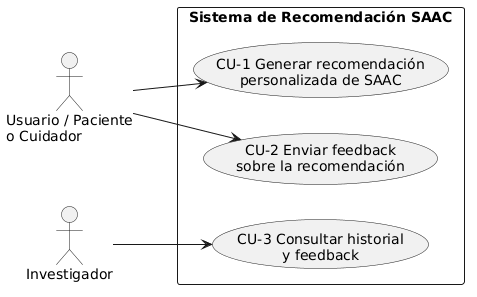
\includegraphics[width=0.85\linewidth]{../img/diagrama_casos_uso.png}
    \caption{Diagrama de Casos de Uso del sistema.}
    \label{fig:casos_uso}
\end{figure}

\section{Explicación casos de uso.}

\begin{table}[ht]
	\centering
	\begin{tabular}
		\toprule
		\textbf{CU-1} & \textbf{Generar recomendación personalizada de SAAC}\\
		\toprule
		\textbf{Versión}  & 1.0    \\
		\textbf{Autor} & [Lucía Gil Aire] \\
		\textbf{Requisitos asociados} & RF-01 (Captura de perfil), RF-02 (Filtrado clínico), RF-03 (Cumplimiento RGPD) \\
		\textbf{Descripción}  & El sistema procesa las capacidades funcionales, entorno y preferencias del usuario para devolver una propuesta de sistemas y periféricos, gestionando de forma segura su consentimiento legal. \\
		\textbf{Precondición} & El usuario debe haber completado los campos obligatorios del formulario y marcado la casilla de aceptación de procesamiento de datos en tiempo real. \\
		\textbf{Acciones}   &
		\begin{enumerate}
			\item El usuario rellena los campos delcuestionario (idioma, capacidades, métodos de entrada, alfabetización, plataformas y entorno de uso).
			\item El usuario envía el formulario mediante una petición POST a la ruta \texttt{/recomendar}.
			\item El sistema valida el consentimiento RGPD obligatorio.
			\item El algoritmo aplica el filtrado clínico en la base de datos comparando las capacidades del usuario con los requisitos mínimos del sistema SAAC.
			\item El sistema ejecuta la función recursiva para asociar periféricos y hardware necesario eliminando duplicados.
			\item Si el usuario autorizó el uso para investigación, el sistema almacena el perfil clínico en formato JSON de forma anónima en la tabla de historial, identificando si se trata de un caso real o de prueba.
			\item El sistema renderiza la plantilla de resultados dividiendo los sistemas finales, preventivos y bancos de voz.
		\end{enumerate}\\
		\textbf{Postcondición}  & Se muestra la pantalla de resultados y, si hubo consentimiento, se genera un registro en la base de datos con un ID anónimo único. \\
		\textbf{Excepciones}  & El usuario no marca la casilla de procesamiento obligatorio: el sistema no procesa el cuestionario y solicita la aceptación del término. \\
		\textbf{Importancia}   & Crítica. \\
		\bottomrule
	\end{tabular}
	\caption{CU-1 Generar recomendación personalizada de SAAC.}
\end{table}

\begin{table}[ht]
	\centering
	\begin{tabular}
		\toprule
		\textbf{CU-2} & \textbf{Enviar retroalimentación (Feedback) sobre la recomendación}\\
		\toprule
		\textbf{Versión}  & 1.0    \\
		\textbf{Autor}   & [Lucía Gil Aire] \\
		\textbf{Requisitos asociados} & RF-04 (Captura de feedback), RF-05 (Vinculación con historial) \\
		\textbf{Descripción}  & El usuario (paciente o cuidador) evalúa la propuesta generada por el sistema y envía un formulario de opinión que se asocia directamente a su registro previo en la base de datos. \\
		\textbf{Precondición}   & El usuario debe haber generado una recomendación previamente, contar con un ID de historial (\texttt{historial\_id}) activo en la sesión y encontrarse en la página de resultados. \\
		\textbf{Acciones}  &
		\begin{enumerate}
			\item El usuario rellena los campos del formulario de feedback (satisfacción, uso actual, motivos de cambio y comentarios).
			\item El usuario envía el formulario mediante una petición POST a la ruta \texttt{/guardar-feedback}.
			\item El sistema recupera el identificador del historial enviado de forma oculta en el formulario.
			\item El sistema busca el registro correspondiente en la tabla \texttt{HistorialRecomendacion} utilizando el método de obtención por clave primaria.
			\item Si el registro existe, el sistema mapea las respuestas en un diccionario estructurado y lo asigna al campo \texttt{feedback}.
			\item El sistema notifica explícitamente el cambio al ORM mediante la instrucción \texttt{flag\_modified} para asegurar la persistencia del objeto JSON.
			\item El sistema realiza el \texttt{db.session.commit()} y renderiza la plantilla de agradecimiento.
		\end{enumerate}\\
		\textbf{Postcondición} & El campo de feedback del registro del historial se actualiza en la base de datos y se muestra la pantalla \texttt{gracias\_feedback.html}. \\
		\textbf{Excepciones} & El identificador del historial no se encuentra en la base de datos o la petición no incluye el ID: el sistema aborta el guardado y muestra la pantalla de agradecimiento estándar de forma segura. \\
		\textbf{Importancia} & Media-Alta (Crítica para el análisis de resultados del TFG). \\
		\bottomrule
	\end{tabular}
	\caption{CU-2 Enviar retroalimentación (Feedback) sobre la recomendación.}
\end{table}

\begin{table}[ht]
	\centering
	\begin{tabular}
		\toprule
		\textbf{CU-3} & \textbf{Consultar historial y feedback de recomendaciones}\\
		\toprule
		\textbf{Versión}   & 1.0    \\
		\textbf{Autor}  & [Lucía Gil Aire] \\
		\textbf{Requisitos asociados} & RF-06 (Visualización de registros), RF-07 (Auditoría e investigación) \\
		\textbf{Descripción} & El investigador del proyecto accede a un panel donde se listan de forma cronológica todas las evaluaciones guardadas, diferenciando los casos de uso clínico real de las pruebas. \\
		\textbf{Precondición}  & Deben existir registros almacenados en la tabla de historial con el consentimiento de investigación otorgado por los usuarios. \\
		\textbf{Acciones}  &
		\begin{enumerate}
			\item El investigador solicita la ruta de administración mediante una petición GET a \texttt{/admin\_historial}.
			\item El sistema realiza una consulta a la base de datos sobre el modelo \texttt{HistorialRecomendacion}.
			\item El sistema ordena los registros de forma descendente utilizando el ID del historial para priorizar los casos más recientes.
			\item El sistema inyecta la lista completa de objetos en la plantilla \texttt{admin\_historial.html}.
			\item El motor de plantillas (Jinja2) procesa de forma iterativa cada registro en la tabla HTML.
			\item Para cada elemento, el sistema evalúa la variable booleana \texttt{es\_real}. Si es afirmativa, renderiza la etiqueta visual «PACIENTE REAL»; en caso contrario, renderiza «PRUEBA / OTROS».
		\end{enumerate}\\
		\textbf{Postcondición} & El investigador visualiza la tabla completa con el identificador anónimo del paciente, fecha, hora, parámetros clínicos, sistemas recomendados y los bloques de feedback si estuvieran rellenados. \\
		\textbf{Excepciones}  & La base de datos está vacía: el sistema renderiza la tabla vacía sin romper la interfaz de usuario. \\
		\textbf{Importancia}  & Alta (Esencial para la consulta de datos de la investigación). \\
		\bottomrule
	\end{tabular}
	\caption{CU-3 Consultar panel de administración del historial.}
\end{table}

\section{Prototipos de interfaz o interacción con el proyecto.}

\section{Interacción del usuario con el cuestionario}
\begin{figure}[htbp]
    \centering
    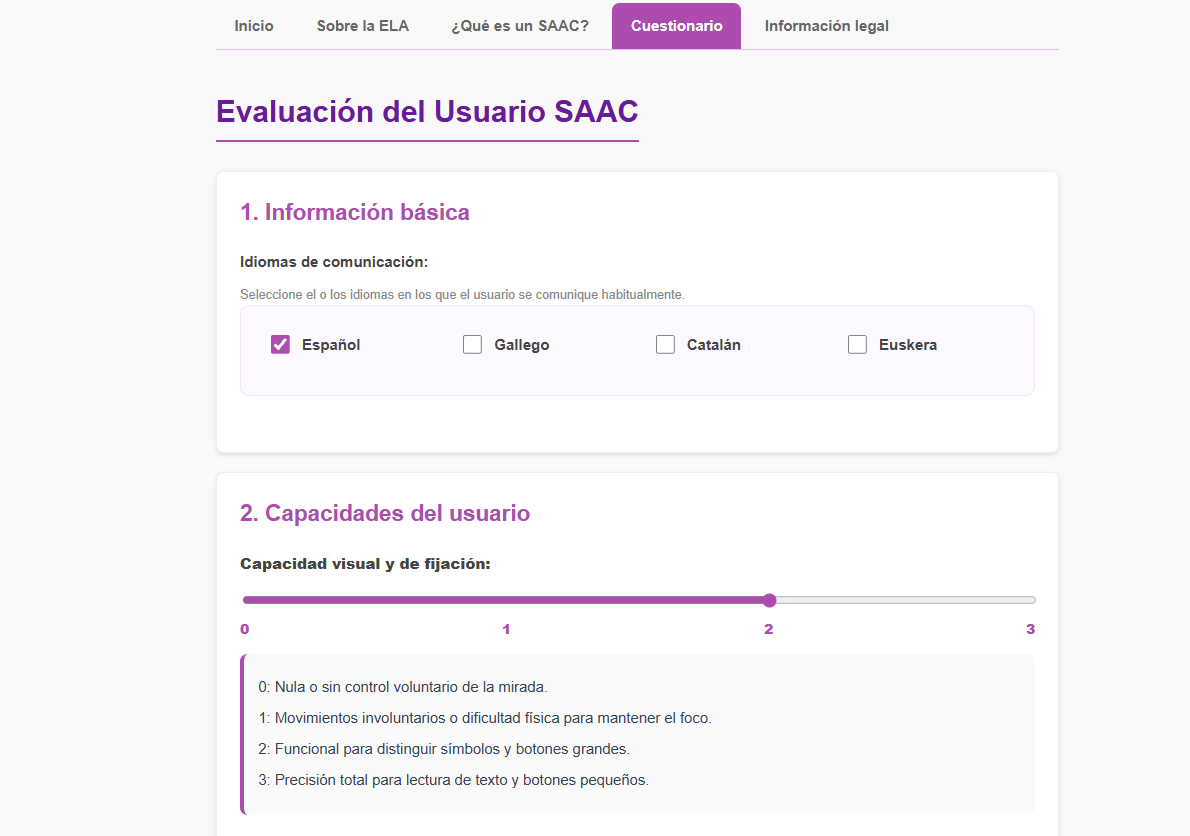
\includegraphics{../img/respuesta_cuestionario_1.png}
    \caption{Respuesta del cuestionario parte I.}
    \label{fig:respuesta_cuestionario_1}
\end{figure}

\begin{figure}[htbp]
    \centering
    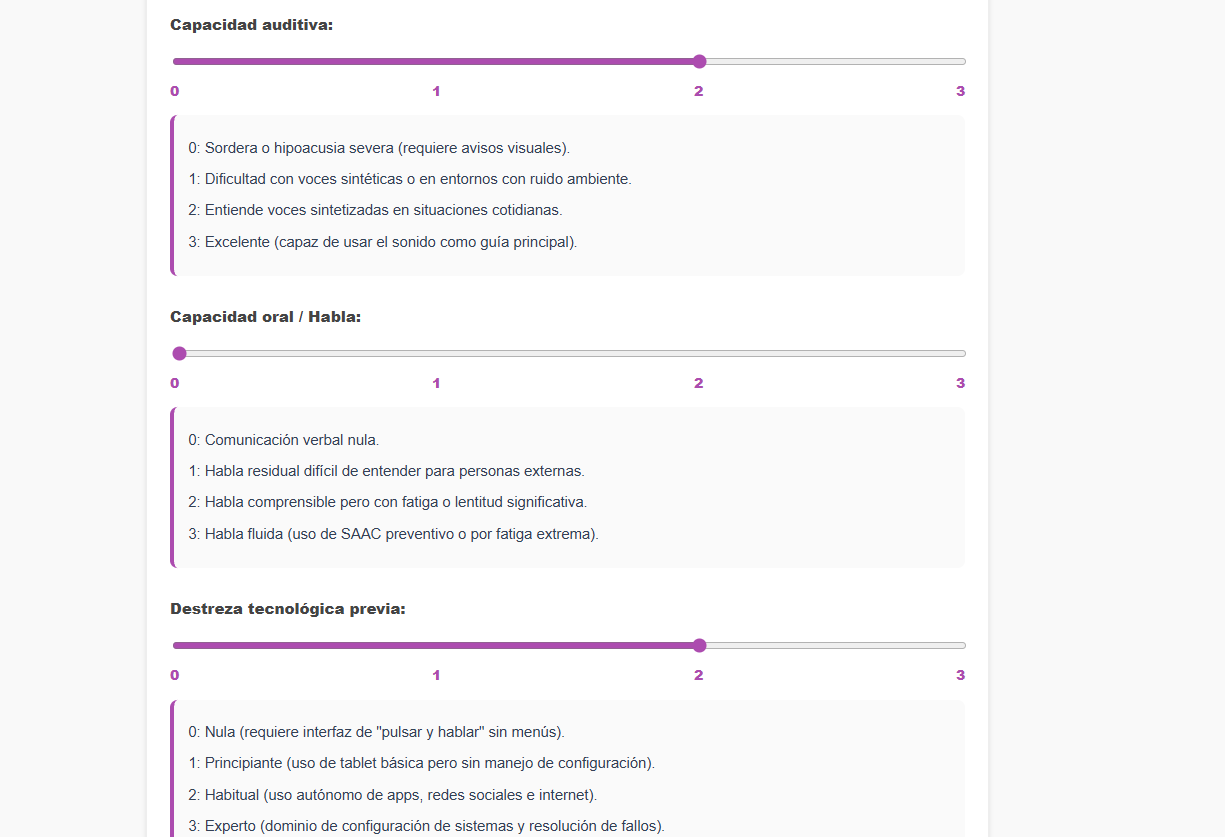
\includegraphics{../img/respuesta_cuestionario_2.png}
    \caption{Respuesta del cuestionario parte II.}
    \label{fig:respuesta_cuestionario_2}
\end{figure}

\begin{figure}[htbp]
    \centering
    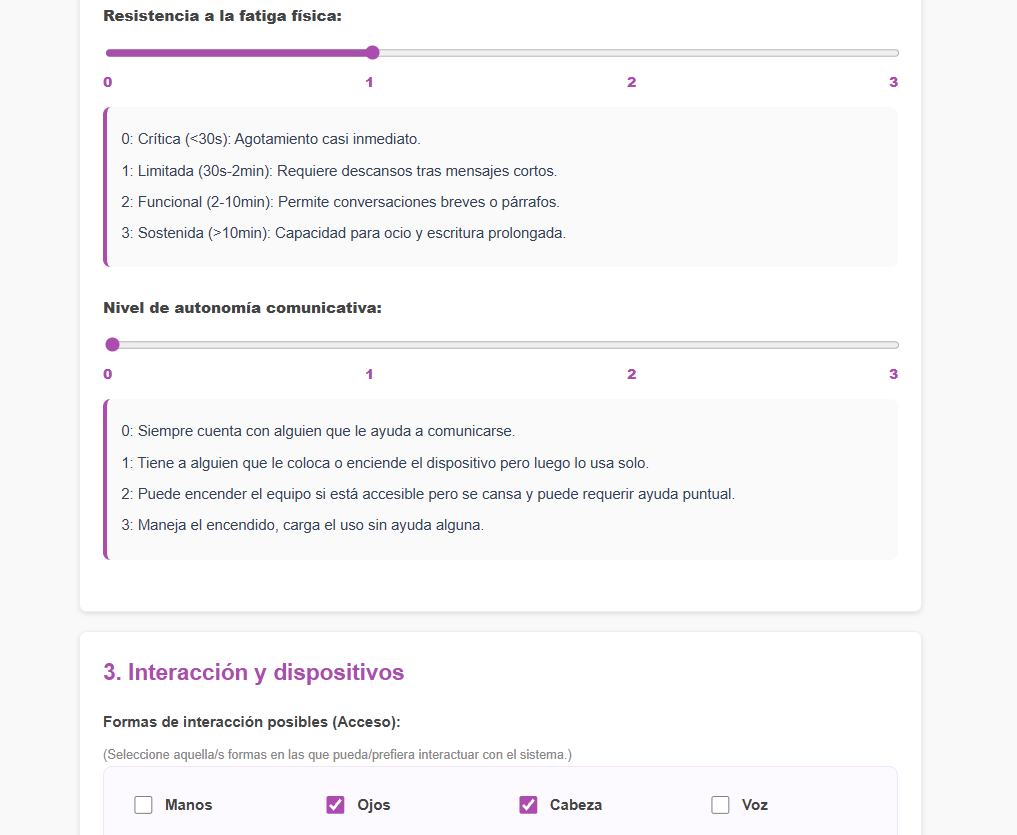
\includegraphics{../img/respuesta_cuestionario_3.png}
    \caption{Respuesta del cuestionario parte III.}
    \label{fig:respuesta_cuestionario_3}
\end{figure}

\begin{figure}[htbp]
    \centering
    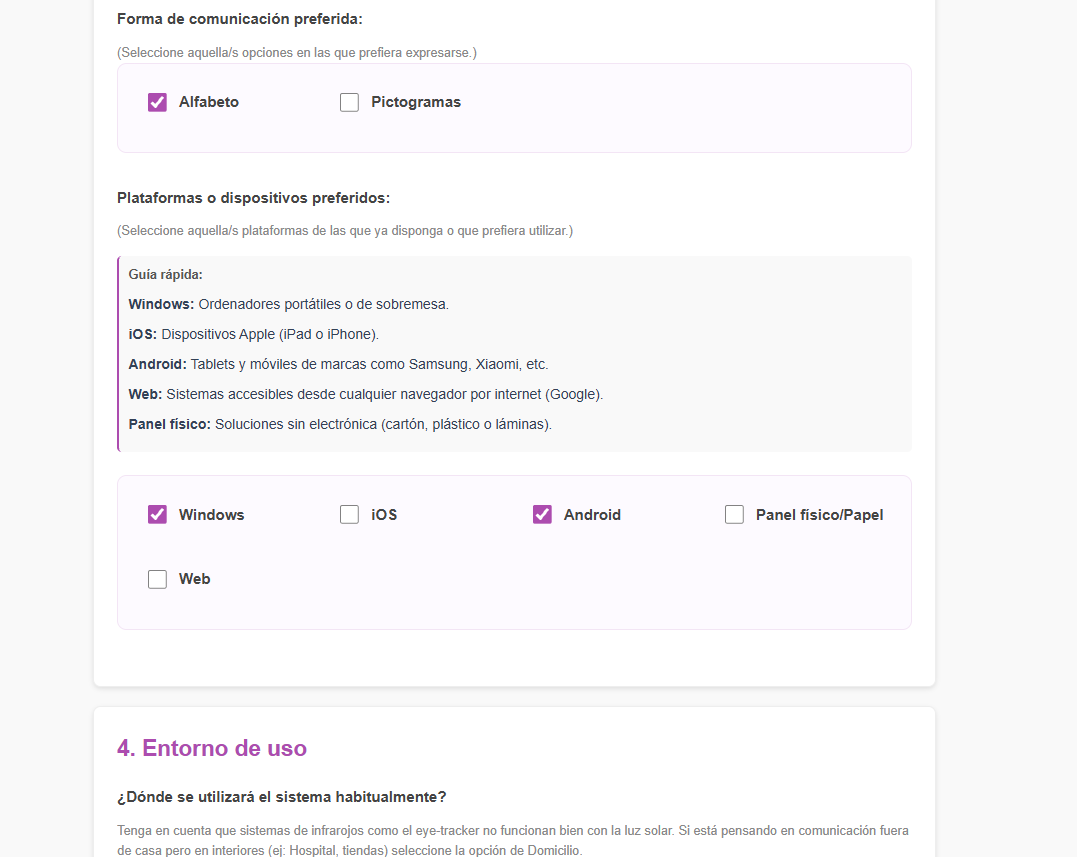
\includegraphics{../img/respuesta_cuestionario_4.png}
    \caption{Respuesta del cuestionario parte IV.}
    \label{fig:respuesta_cuestionario_4}
\end{figure}

\begin{figure}[htbp]
    \centering
    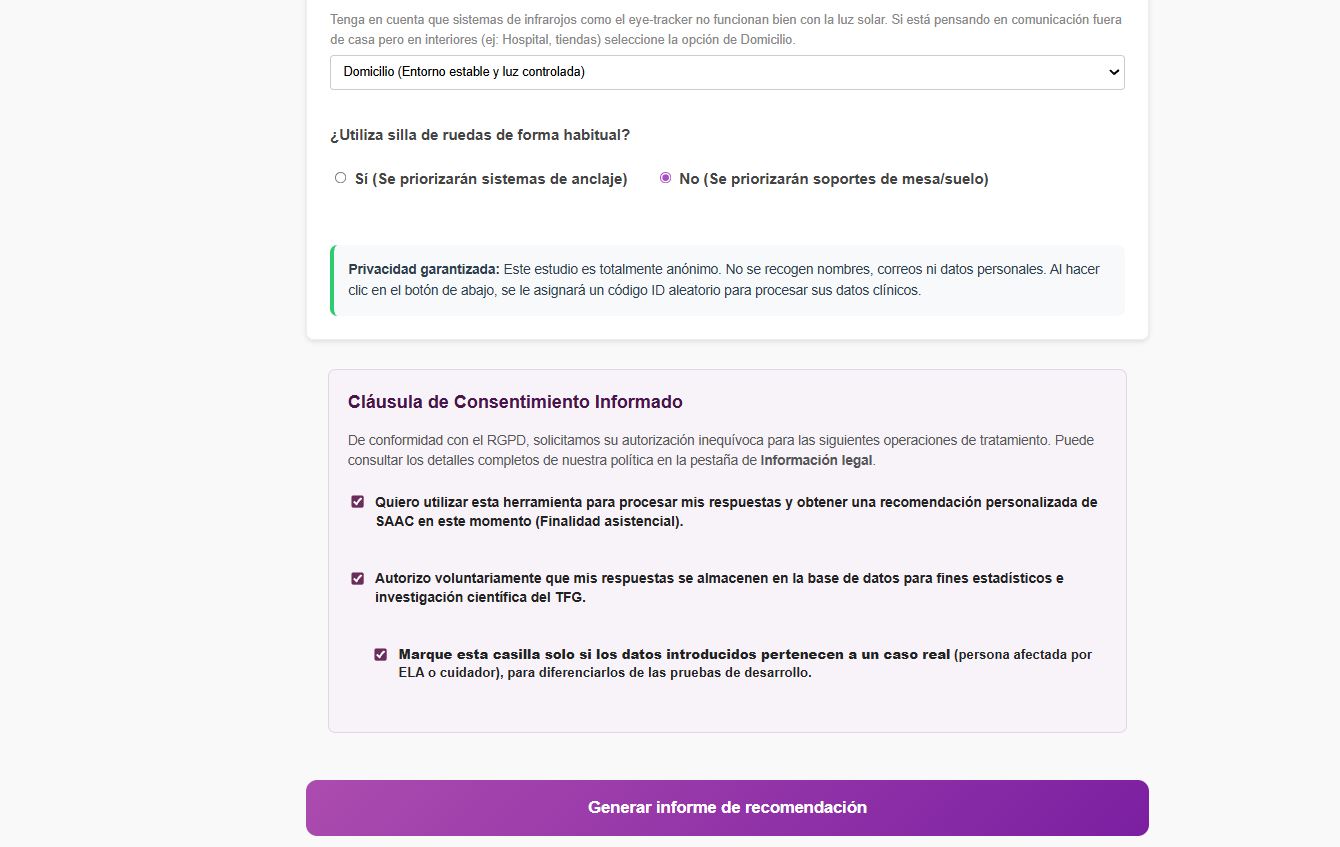
\includegraphics{../img/respuesta_cuestionario_5.png}
    \caption{Respuesta del cuestionario parte V.}
    \label{fig:respuesta_cuestionario_5}
\end{figure}


